\section{Результаты работы тренировки}

\subsection{Вариант 0}

По умолчанию выставлен задач планирования --- фиксированный объем рессурсов.

\begin{figure}[ht!]
	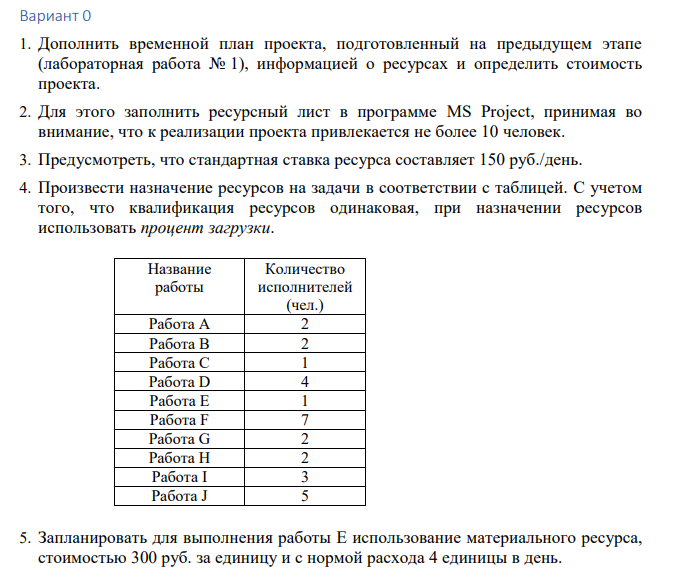
\includegraphics[width=0.75\linewidth]{assets/images/image_2024-02-27_09-41-29.png}
	\label{fig:r2}
	\caption{Задание тренировки}
\end{figure}
\FloatBarrier

\begin{figure}[ht!]
	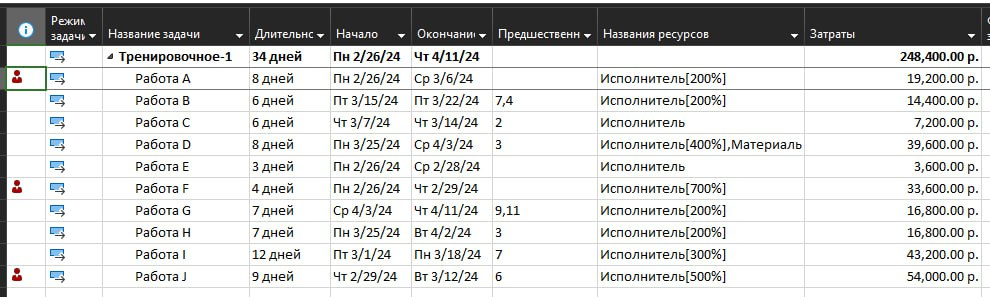
\includegraphics[width=\linewidth]{assets/images/task2.jpg}
	\label{fig:r2}
	\caption{Резульатат тренировочного задания}
\end{figure}
\FloatBarrier

\section{Результаты работы второй лабораторной работы}

\subsection{Создание списка ресурсов}

\begin{figure}[ht!]
	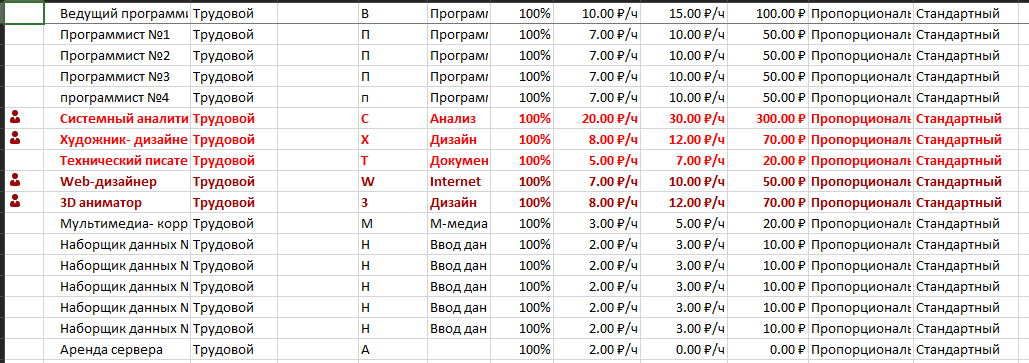
\includegraphics[width=0.75\linewidth]{assets/images/image_2024-02-27_09-33-23.png}
	\label{fig:r2}
	\caption{Ресусры}
\end{figure}
\FloatBarrier

\subsection{Назанчение ресурсов задачам}

\begin{figure}[ht!]
	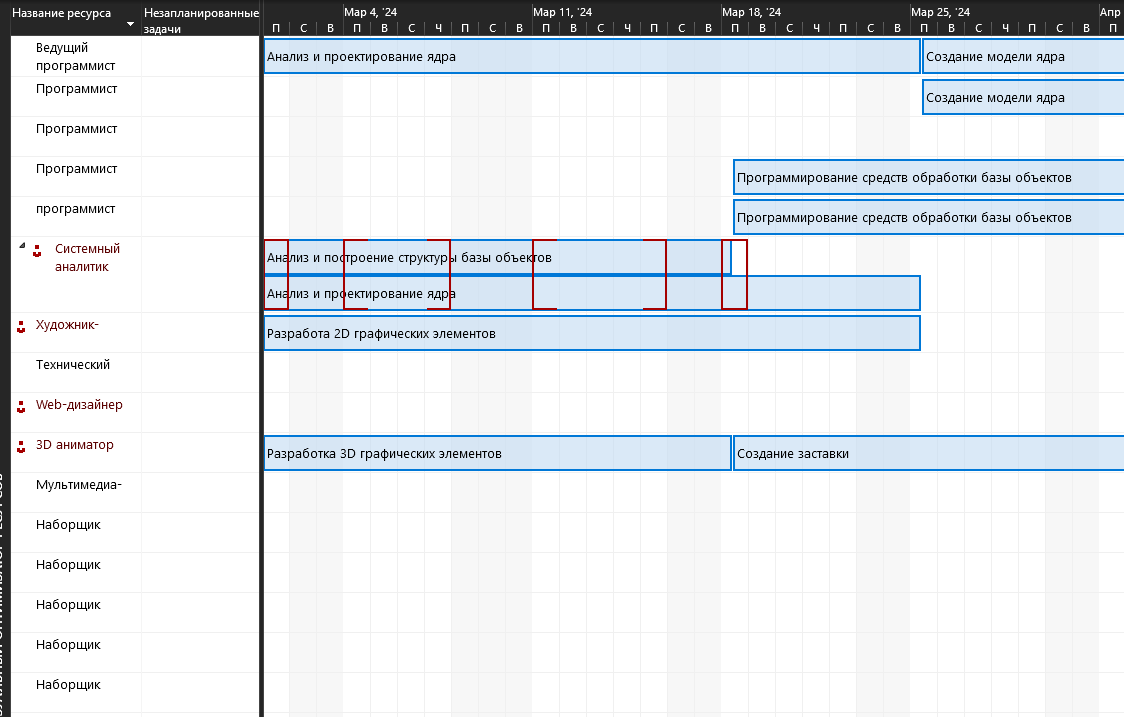
\includegraphics[width=0.75\linewidth]{assets/images/image_2024-02-27_09-35-16.png}
	\label{fig:r2}
	\caption{Ресусры}
\end{figure}
\FloatBarrier

Видно, что у художника-дизайнера задачи накладываются друг на друга и он не успевает их выполнить.

\begin{figure}[ht!]
	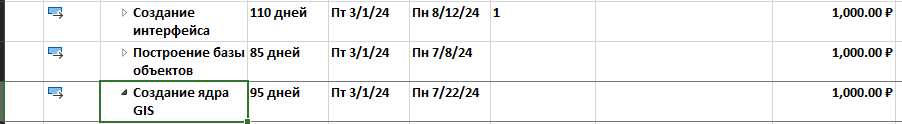
\includegraphics[width=0.75\linewidth]{assets/images/image_2024-02-27_09-35-44.png}
	\label{fig:r2}
	\caption{Ресусры}
\end{figure}
\FloatBarrier

\subsection{Анализ затрат по группам ресурсов}

\begin{figure}[ht!]
	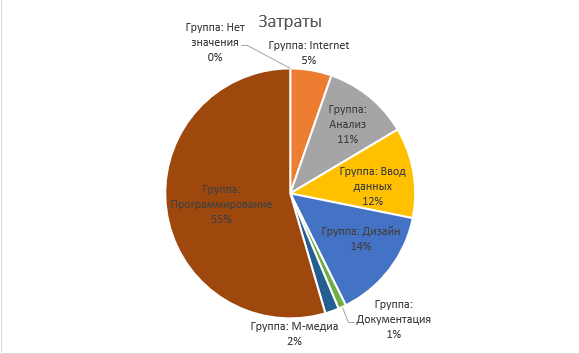
\includegraphics[width=0.75\linewidth]{assets/images/image_2024-02-27_11-16-29.png}
	\label{fig:r2}
	\caption{Затраты}
\end{figure}
\FloatBarrier

\begin{figure}[ht!]
	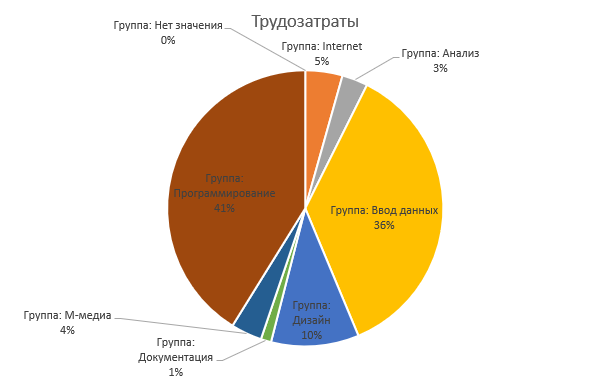
\includegraphics[width=0.75\linewidth]{assets/images/image_2024-02-27_11-17-48.png}
	\label{fig:r2}
	\caption{Трудозатраты}
\end{figure}
\FloatBarrier

\subsection*{Вывод}

Согласно диаграммам, можно сделать вывод, что наиболее затратная работа прораммистов, сервера, ввод данных и анализа.
У программистов и аналитиков наибольшее соотношение затарат к трудозатратам.
Обратная ситуация наблюдается у сервера.